
\documentclass[11pt,letterpaper]{article}


\usepackage{blindtext} 
\usepackage{graphicx}
\usepackage[sc]{mathpazo} 
\usepackage[T1]{fontenc} 
\linespread{1.05} 
\usepackage{microtype} 


\usepackage[english]{babel} 


\usepackage[hmarginratio=1:1,top=32mm,columnsep=20pt]{geometry} 
\usepackage[hang, small,labelfont=bf,up,textfont=it,up]{caption} 
\usepackage{booktabs} 


\usepackage{lettrine} 


\usepackage{enumitem} 
\setlist[itemize]{noitemsep} 


\usepackage{abstract} 
\renewcommand{\abstractnamefont}{\normalfont\bfseries} 
\renewcommand{\abstracttextfont}{\normalfont\small\itshape} 


\usepackage{titlesec} 
\renewcommand\thesection{\Roman{section}} % 
\renewcommand\thesubsection{\roman{subsection}} 
\titleformat{\section}[block]{\large\scshape\centering}{\thesection.}{1em}{} 
\titleformat{\subsection}[block]{\large}{\thesubsection.}{1em}{} 


\usepackage{fancyhdr} 
\pagestyle{fancy} 
\fancyhead{} 
\fancyfoot{} 
\fancyhead[C]{Principios de diseño y DDD $\bullet$ Septiembre 2021 $\bullet$ } 
\fancyfoot[RO,LE]{\thepage} 


\usepackage{titling} 


\usepackage{hyperref} 


%----------------------------------------------------------------------------------------
%	TILULOS
%----------------------------------------------------------------------------------------


\setlength{\droptitle}{-4\baselineskip} 

\pretitle{\begin{center}\Huge\bfseries} 
\posttitle{\end{center}} 
\title{Principios de diseño y DDD} 
\author{André Pómez, Diego Gorbeño, Brian Anco, Ericka Martínez, Alfredo Huillca y Midwar Loza }
\date{\today} 
\renewcommand{\maketitlehookd}{

\begin{abstract}
\noindent 
Design is one of the important phases of the software development lifecycle, if the design is good, all other phases of the software development lifecycle, such as coding, maintenance and support, will be stress and hassle free. Today's agile development world has driven the developer to compete with the latest features and technologies in the market. However, it is difficult for naïve users to maintain design quality if there are no standard guidelines available.\\
Sometimes the quality of the design depends solely on the developer's experience, so we must have standard and proven design guidelines to work. If the software design is in accordance with the principles and patterns, it can increase the reusability, maintainability and scalability of the software, so this research paper focuses on describing and explaining the SOLID design principle and domain driven design (DDD), thus highlighting their concepts, features, advantages, disadvantages and uses.\\\\

\end{abstract}
\section{Resumen}


El diseño es una de las fases importantes del ciclo de vida del desarrollo de software, si el diseño es bueno, todas las demás fases del ciclo de vida del desarrollo de software, como la codificación, el mantenimiento y el soporte, serán sin estrés y sin complicaciones. El mundo del desarrollo ágil actual ha llevado al desarrollador a competir con las últimas funciones y tecnologías del mercado. Sin embargo, para los usuarios ingenuos es difícil mantener la calidad del diseño si no hay pautas estándar disponibles. \\
En ocasiones, la calidad del diseño depende únicamente de la experiencia del desarrollador, por lo que debemos tener guías de diseño estándar y comprobadas para funcionar. Si el diseño del software está de acuerdo con los principios y patrones, puede aumentar la capacidad de reutilización, mantenimiento y escalabilidad del software, por lo que este artículo de investigación se centra en la descripción y explicación del principio de diseño SOLID y el diseño impulsado por dominio (DDD), resaltando así sus conceptos, características, ventajas, desventajas y usos.
\\\\


}

%----------------------------------------------------------------------------------------

\begin{document}

% Print the title
\maketitle

%----------------------------------------------------------------------------------------
%	INTRODUCCION
%----------------------------------------------------------------------------------------

\section{INTRODUCCIÓN}
\lettrine[nindent=0em,lines=3]{E}
l diseño del software ayuda a imaginar el sistema global y reduce el coste de desarrollo y soporte del proyecto. Dado que no es fácil identificar la viabilidad de los requisitos reales al principio del proyecto, por lo tanto, el diseño debe soportar la escalabilidad que permitirá la inducción de los nuevos requisitos en la arquitectura del software. Para apoyar la escalabilidad hay algunos factores importantes en los que el diseñador debe concentrarse mientras piensa en el diseño del software para evitar el rediseño.\\
Estos factores son la rigidez, la fragilidad, la inmovilidad y la viscosidad. La rigidez especifica la medida de dificultad para cambiar el software. La fragilidad es la tendencia del software a romperse cada vez que se modifica. La inmovilidad es la incapacidad de reutilizar software de otros proyectos o partes de software del mismo proyecto. La viscosidad es la incapacidad de preservar el diseño del sistema, que puede degradarse si no se incorpora una solución adecuada a cualquier cambio en los requisitos del sistema.\\
La presencia de estos cuatro factores da lugar a una arquitectura deficiente. Cualquier aplicación que presente estos factores está sufriendo un mal diseño. Para manejar estos factores tenemos un conjunto de directrices llamadas Principios de Diseño. Este articulo presenta una la descripción y explicación del principio de diseño SOLID, relacionado con la comprensión y el uso de patrones de diseño que permite mantener una alta cohesión y por lo tanto, un bajo acoplamiento de software y el diseño impulsado por dominio (DDD) un modelo rico, expresivo y en constante evolución que busca resolver problemas del dominio de una forma semántica que podrán ayudar a tomar decisiones de diseño con el fin de enfocar y acelerar el manejo de dominios complejos durante el desarrollo de proyectos digitales. 
\\\\




\section{DESARROLLO}


\subsection{Principios S.O.L.I.D.} 

\textbf{ 1.1. Principio de responsabilidad única } 
\\El Single Responsibility Principle (SRP) o principio de responsabilidad única es un principio que defiende que una clase o módulo debería tener responsabilidad sobre una única funcionalidad del software.
Robert C. Martin define el principio con la siguiente frase: “Una clase debe tener solo una razón para cambiar.”. No queremos que una misma pieza de código tenga que cambiar debido a personas distintas ya que las personas son las que dirigen los cambios en el software. Por ejemplo, un cambio en Employee sobre su forma de trabajar vendrá requerido por una persona distinta del que vendrá un cambio sobre la tecnología de persistencia de datos.\\\\\\
EJEMPLO\\
Tenemos que diseñar un supermercado, una primera aproximación podría ser:\\
\begin{center}
	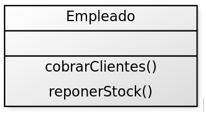
\includegraphics[width=10cm]{./imagenes/1.png} 
\end{center}
Tenemos una clase empleado que puede cobrar a los clientes en la caja registradora, pero también repone el Stock.\\
Si seguimos este principio deberíamos haber hecho un modelo similar a este.\\
\begin{center}
	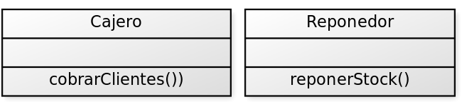
\includegraphics[width=10cm]{./imagenes/2.png} 
\end{center}
Así las peticiones de cambio serán más sencillas de implementar y una nueva incorporación al equipo de desarrollo no tendrá tantos problemas para entender el código.
\\\\\\
\textbf{ 1.2. Principio abierto/cerrado } 
\\Representa la O de SOLID. Con este principio se pretende minimizar el efecto cascada que puede suceder cuando cambiamos el comportamiento de una clase. Si existen clientes que dependan de ella, es posible que tengan que cambiar su comportamiento también.
Consta de 2 partes:\\\\
{- Las clases deben estar abiertas a la extensión. La extensión se refiere a las modificaciones que pueden ocurrir cuando se plantean nuevos requisitos de software.}\\
{- Las clases deben estar cerradas a la modificación. No se puede cambiar el código fuente de una clase.}
\\\\\\\\\\
EJEMPLO\\
Tenemos una empresa que desde sus comienzos ha estado vendiendo agua embotellada,
y su programa informático tenía esta forma.\\
\begin{center}
	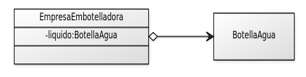
\includegraphics[width=10cm]{./imagenes/3.png} 
\end{center}
Ahora ha surgido una oportunidad de negocio y quiere empezar a vender botellas de té helado, por lo que necesita un cambio en su modelo.\\
Una primera aproximación sería algo similar a esto:\\
\begin{center}
	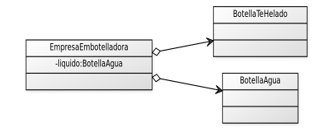
\includegraphics[width=10cm]{./imagenes/4.png} 
\end{center}
Pero implicaría realizar cambios en la empresa, que tiene que aprender a comunicarse con el nuevo tipo de botella, que probablemente sea muy parecida a la anterior.
\begin{center}
	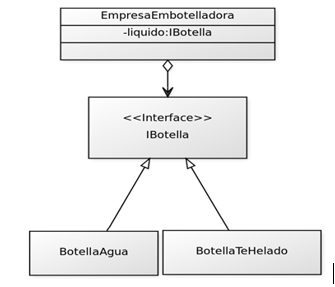
\includegraphics[width=10cm]{./imagenes/5.png} 
\end{center}

\textbf{ 1.3. Principio de sustitución de Liskov}
\\Introducido por Barbana Liskov, representa la L de los principios S.O.L.I.D. , dice que si la clase A es de un subtipo de la clase B, entonces deberíamos poder reemplazar B con A sin afectar el comportamiento de nuestro programa.
Hay una frase muy conocida que dice “Si se ve como un pato, hace cuac como un pato, pero necesita baterías, probablemente tengas la abstracción incorrecta”.
Si tenemos una clase que hereda de otra, pero hay un método que no se necesita o no se usa en esa clase. Para solucionar esto, podriamos devolver null o una excepción en ese método. Al hacer esto, estamos violando el Principio de Sustitución de Liskov. Si el método de la clase original no lanza ninguna excepción, los métodos sobrescritos de las subclases tampoco deberían hacerlo.
\\ \\ 
\textbf{ 1.4. Principio de segregación de interfaces}
\\Este principio es bastante fácil de comprender, defiende dice que ningún cliente debería estar obligado a depender de los métodos que no utiliza.
En una interfaz existente no debería agregar nuevos métodos que obliguen a implementar funcionalidad adicional. En vez de agregar métodos a una interfaz existente, es mejor crear otra interfaz y que la clase que la necesite la implemente.
Cuando creamos una interfaz debemos estar seguros de que la clase que va a implementar la interfaz va a poder implementar todos los métodos.
Por lo general siempre será preferible muchas interfaces pequeñas a una gran interfaz con muchos métodos.
\\ \\ 
\textbf{ 1.5. Principio de inversión de dependencias}
\\El principio tiene como fin evitar depender de concreciones para minimizar el grado de acoplamiento entre los componentes.\\
Ventajas:\\\\
- Reduce el acoplamiento entre clases: al no depender de una implementación en concreto, no acoplamos nuestro código a ciertas clases específicas.\\
- Código más limpio, legible y mantenible en el tiempo: al no depender de implementaciones, estamos contribuyendo a un desarrollo más robusto y que no sea frágil a cualquier cambio.\\
- Al depender de abstracciones, tenemos la posibilidad de elegir en tiempo de ejecución la implementación adecuada.
\\ \\ 


\subsection{Domain Driven Desing}
DDD se ocupa tanto del desafío de comprender el problema de un dominio como de crear
una solución mantenible que sea útil para resolver problemas dentro de él. El lenguaje
común, la colaboración con los expertos del dominio y el contexto, se consideran las facetas
más importantes del DDD.  \\
Las cuatro capas de la arquitectura DDD representan:\\\\
\textbf{ - Capa presentación } 
\\ Es el Interfaz de usuario, responsable de presentar e interactuar con la
información del usuario\\\\
\textbf{ - Capa de Aplicación } 
\\Coordina la actividad de la aplicación. No contiene ninguna lógica
empresarial, ni estado de los objetos comerciales, pero puede contener el estado del
progreso de una tarea de aplicación\\\\
\textbf{ - Capa de dominio } 
\\ Contiene información sobre el dominio empresarial. El estado de los
objetos comerciales se mantiene aquí \\\\
\textbf{ - Capa de infraestructura } 
\\Actúa como una biblioteca de apoyo para todas las demás capas.
Proporciona comunicación entre capas, implementa persistencia para objetos comerciales,
contiene bibliotecas de soporte para la capa de interfaz de usuario, etc.
\\\\
Dentro de DDD encontramos muchos conceptos y patrones. Estos se pueden dividir en dos
tipos:\\
\textbf{ Patrones estratégicos } 
\\Destilan el problema del dominio y dan forma a la arquitectura de la
solución. Van a definir como se comunican e interactúan los desarrolladores con los
expertos del dominio, un idioma común que emplear, límites de contexto, mapas de
contextos e interrelaciones, y en general todas las cuestiones que no atañen directamente
al código de la aplicación
\\\\
\textbf{ Patrones tácticos } 
\\También conocidos como bloques de construcción de modelos, son los
patrones que atañen a todo lo referente al código de la solución y se utilizan para
implementar modelos efectivos para contextos delimitados complejos
\\\\




  \section{CONCLUSIONES}
 Aplicar el S.O.L.I.D nos da una gran ventaja al momento de realizar nuestro código, abarcando la fase de mantenimiento de una manera más legible y sencilla así como conseguir crear nuevas funcionalidades sin tener que modificar en gran medida código antiguo.\\\\
El S.O.L.I.D. también ayuda a categorizar lo que es un buen código limpio o de uno malo, salvo en ciertos casos, ya que no hay pruebas que siempre funcione o de que siempre se deba seguir.\\\\
A pesar de que los principios del S.O.L.I.D. son considerados por muchos como una base fundamental de un buen desarrollo, podría tener ciertas desventajas como la de ser ambiguos, confusos, de complicar el código o de demorar el proceso de desarrollo.\\\\
DDD pone un énfasis especial en el análisis, el enfoque en el dominio principal y la
comunicación y colaboración entre los desarrolladores y los expertos del dominio. Conforme
van siendo los desarrollos más complejos y más relevantes se muestran estos patrones
estratégicos.\\


\section{RECOMENDACIONES}
Hay muchos principios en la ingeniería de software y se recomendaría que antes de escribir
un código, hay que indagar un poco sobre ello, leer e intentar entender sus principios.\\
Aunque pueda parecer mucho, SOLID se convierte en una parte de ti y tu codigo utilizandolo
con continuidad y adaptándose a sus guías.\\
El ámbito del desarrollo de software es un terreno de continuo debate y SOLID no se queda
fuera de la controversia.\\
Aunque estos cinco principios son considerados por muchos como una base fundamental
de un buen desarrollo o al menos como una guía a tener en cuenta, no son pocos los
profesionales que critican los principios SOLID.\\
Los acusan de ambiguos, confusos, de complicar el código, de demorar el proceso de
desarrollo y los tildan incluso de totalmente equivocados e innecesarios.\\
Por otro lado, DDD es independiente del lenguaje de programación elegido, no requiere el
uso de ningún frameware o base de datos especial, ni impone el uso de una arquitectura
específica para el desarrollo. Una metodología orientada a objetos es útil para construir los
modelos, aunque tampoco es un requerimiento obligatorio.


\begin{thebibliography}{99} % Bibliography - this is intentionally simple in this template

\bibitem.Chebanyuk E  Markov K (2016 February)
\newblock An approach to class diagrams verification according to SOLID design principles. In 2016 4th International Conference on Model-Driven Engineering and Software Development

\bibitem.Hippche B Giessler P Steinegger R Schneider M  Abeck S (2017).
\newblock Designing microservice-based applications by using a domain-driven design approach International Journal on Advances in Software (1942-2628) 10(12) 2017

\bibitem
.Landre E Wesenberg H  Olmheim J (2007, October).
\newblock Agile enterprise software development using domain-driven design and test first In Companion to the 22nd ACM SIGPLAN conference on Object-oriented programming systems and applications companion (pp 983-993)
	
\bibitem .Le D M Dang D H  Nguyen V H (2020).
\newblock Generative software module development for domain-driven design with annotation-based domain specific language Information and Software Technology 120 106239.

\bibitem .Madasu V K Venna T V S N Eltaeib T Moalla M A Almuslet N A Badaoui A Lufi B.
\newblock SOLID Principles in Software Architecture and Introduction to RESM Concept in OOP Studies 35(38) 8. 

\bibitem .Nagy T (2019, October).
\newblock Western Canon of Software Engineering: The Abstract Principles In 2019 10th IEEE International Conference on Cognitive Infocommunications (CogInfoCom) (pp 153-156) IEEE. 

\bibitem .Oktafiani I  Hendradjaya B (2018, November).
\newblock Software Metrics Proposal for Conformity Checking of Class Diagram to SOLID Design Principles In 2018 5th International Conference on Data and Software Engineering (ICoDSE) (pp 1-6) IEEE. 

 \bibitem .Rademacher F Sorgalla J  Sachweh S (2018).
\newblock Challenges of domain-driven microservice design: a model-driven perspective IEEE Software 35(3) 36-43.

 \bibitem .Singh H  Hassan S I (2015). 
\newblock Effect of solid design principles on quality of software: An empirical assessment International Journal of Scientific  Engineering Research 6(4).

 \bibitem .Wesenberg H Landre E  Rønneberg H (2006, October).
\newblock Using domain-driven design to evaluate commercial off-the-shelf software In Companion to the 21st ACM SIGPLAN symposium on Object-oriented programming systems languages and applications (pp 824-829).

	
\end{thebibliography}




\end{document}
